
\begin{figure*}
	\centering
	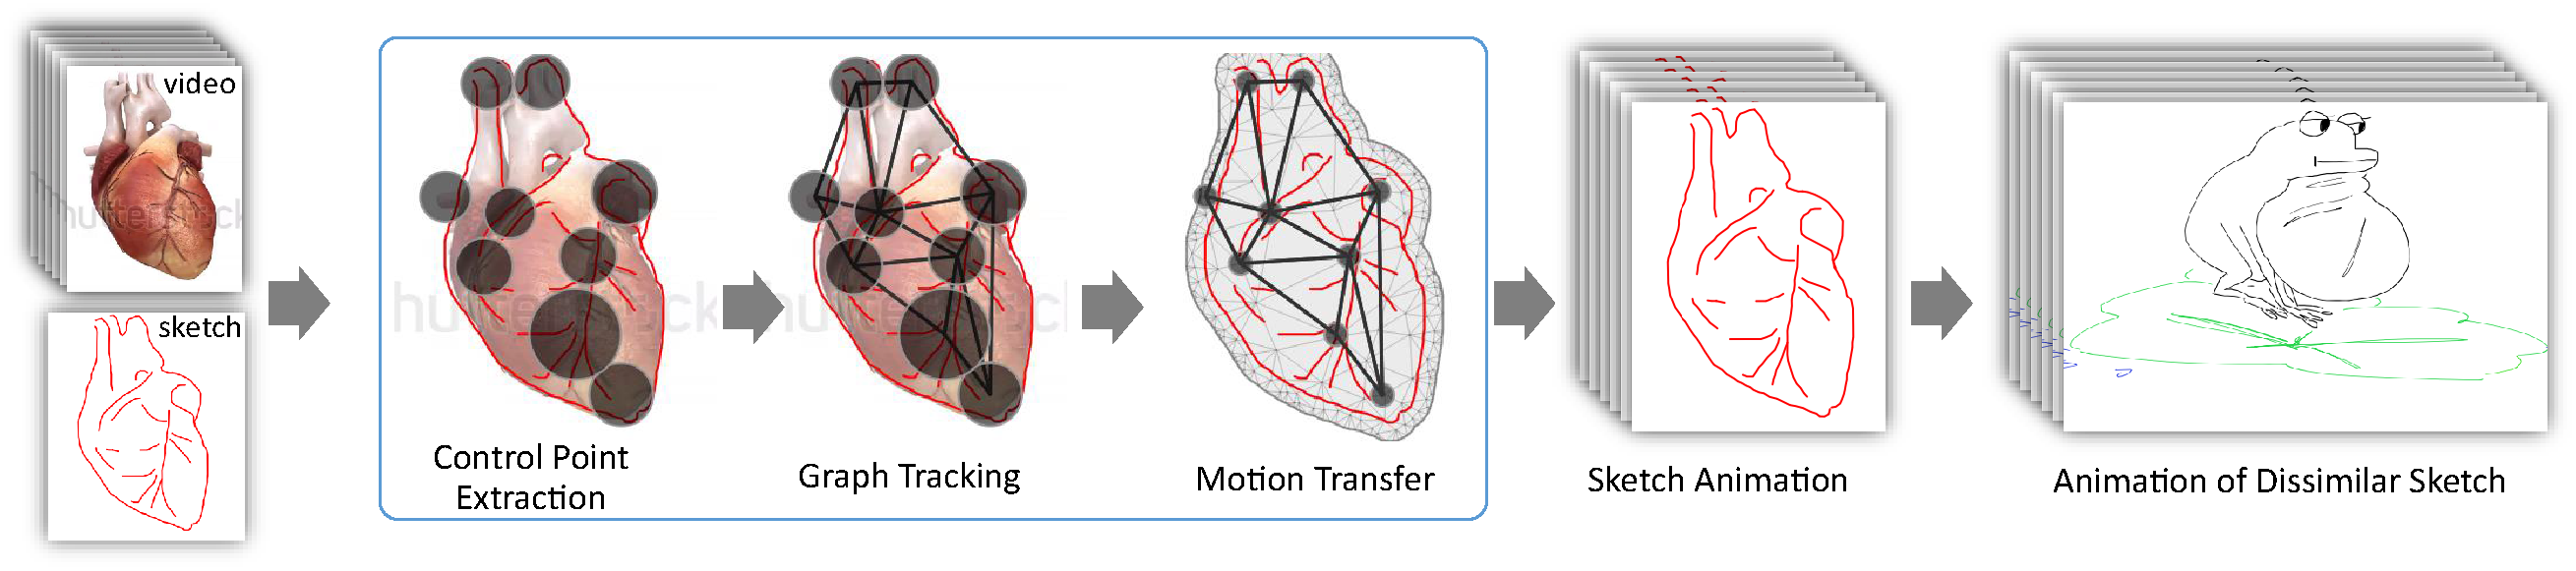
\includegraphics[width=0.85\linewidth]{images/overview}
	\caption{System overview. If the layout is OK, I will change this example to the candle.\jue{for "Sketch animation", can you add multiple frames to represent a sequence?}}
	\label{fig:overview}
\end{figure*}

\section{Our System}

\subsection{System Overview}\label{sec:overview}

Our system takes a static sketch drawing and a video sequence that contains the desired motion for the sketch as input. The moving object should be entirely visible throughout the video. For minimal user interaction, the video object should contain relatively rich texture and has a clear boundary against the background. Let's first assume that the user-provided sketch drawing matches the video object well in shape, so that the correspondence between the image features and sketch lines exist naturally. \ca{This could be achieved (correspondence could be achieved by this?)} by using previous intelligent image-guided sketching interfaces such as EZ-Sketching~\cite{EZSketching:2014}. We will describe in Sec.~\ref{} how to extend the system to handle more creative user sketches that do not necessarily match the shapes of the video objects.  


Our system workflow is shown in Fig.~\ref{fig:overview}. 
Given the input video and sketch drawing, our system first  extracts a series of control points that satisfy two constraints: (1) be easy to track; and (2) be semantically meaningful to guide the sketch deformation to create animation, with the user's help. We then construct an elastic graph using these points as nodes, and track their positions through the video using a novel graph tracking method that jointly considers (1) the tracking accuracy of individual nodes; and (2) the elasticity or rigidity constraints defined on edges between nodes. Given that perfect tracking could be extremely difficult for hard cases, we keep the user in the loop in the tracking process to provide additional guidance. The user can correct tracking errors on keyframes, or specify special geometric constraints between any pair of nodes. The algorithm takes into account the user inputs to produce satisfactory tracking results. 
Finally, the tracked control points are used as guidance to a stroke-preserving mesh deformation algorithm to generate a deformed sketch on each frame, resulting in the final animation. 
We further allow the user to quickly specify local rigidity of mesh deformation for achieving more desirable results. 
%\qingkun{However, some strokes may be distorted by the direct mesh deformation. Therefore, we allow the user to select the strokes by a local rigidity brush. Our system then reconstruct the mesh by adding more triangles which is used for keeping the shape of these strokes. Our method does not add the shape constraint to all strokes because the harder the shape constraint we give, the more motion would be lost.}
In the following sub-sections, we will describe each of the technical components in more detail. 

%
%\begin{figure}
%	\centering
%	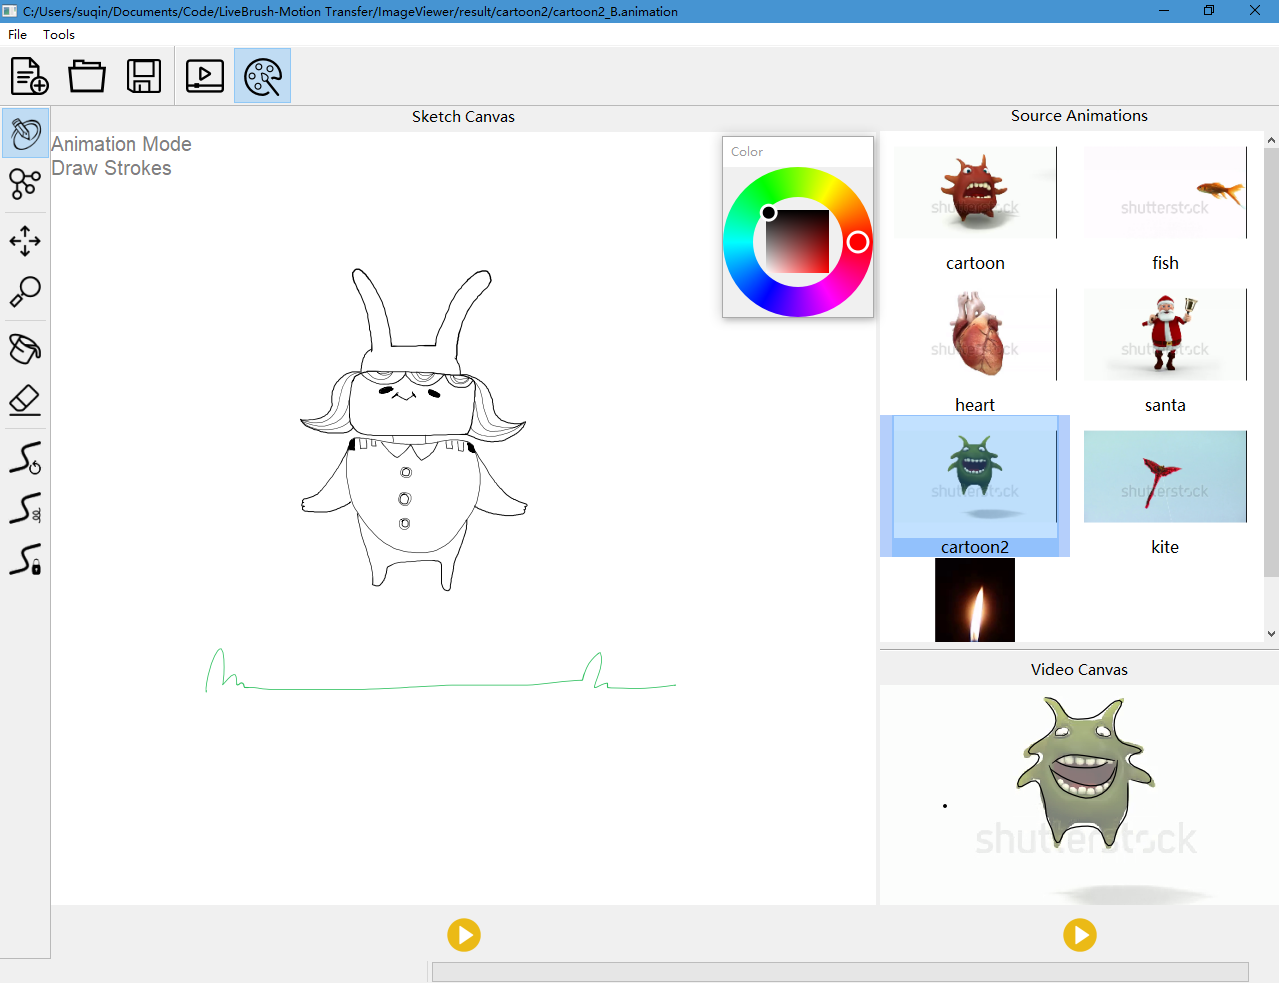
\includegraphics[width=0.85\linewidth]{images/ui}
%	\caption{}
%	\label{fig:ui}
%\end{figure}

\subsection{Control Point Extraction}\label{feature_extraction}

The first step of the system is to extract a set of sparse points on the sketch as ``knobs'' for deforming the sketch for animation. The position of these points are tracked through the video, so object motion is represented by their trajectories. Note that since the primary utility of these points are for controlling animation, commonly used image features such as SIFT or SURF are not desirable, as they describe only local image features rather than semantically meaningful representation of the the object shape. Furthermore, we expect the number of such points to be minimal for reduced tracking complexity and smooth sketch deformation. 
Automatically computing such points is extremely hard, as it requires strong prior knowledge on the motion of the underlying physical object. 
 
We first compute the object region that the control points should be extracted from. This is done by applying the active contour method~\cite{Kass88snakes} on the sketch image to produce an membrane that encloses all sketch strokes.
Inside the object region, we find all the starting and ending points of the strokes, as well as high curvature points along each stroke. These points encode most of the topology information of the sketched object. We group them into clusters based on their spatial distances by using a simple K-Means clustering in 2D space, and use the centroid of each cluster as a control point candidate. The user can additionally move or delete these points, or adding new ones through our interface. 

The user-adjusted control points can well represent the structure of the object, but may not be optimal for tracking. To improve their trackability through the video, we apply a final adjustment step to their positions. For each control point, we use the multi-level Shi-Tomasi corner detection method~\cite{Shi_1994_3266} in its vicinity to compute a local multi-level ``goodness to track'' measure, where the size of the support region in each level, denoted as $r$, is set to be $ r_0, 2r_0, 3r_0 $, with $r_0$ being the 1/10 diagonal length of the sketch bounding box. We then identify the local maximal in this multi-level local measurement map, and move the control point to it. We also record the support region size for each adjusted control point, which will be used in the tracking process. Formally, we describe the supporting image region of a control point as $C_i=\{\mathbf{x}_i, r_i\}$ (i.e., center position and size). $r_i$ is kept as a constant and we seek to determine $\mathbf{x}_i$ in each frame in the tracking process. 


\subsection{Graph Tracking}\label{motion_extraction}

After the control points are determined on the first frame, we track their positions through the video to create motion trajectories that represent the coarse object motion. These trajectories will later be used to guide sketch deformation for final animation. A na\"{i}ve approach to extract them would be to to track each control point individually using traditional computer vision techniques. However, we found such a strategy unsatisfactory, as tracking errors of individual control points often lead to significant distortion of the sketch image. Such an example is shown in Fig.~\ref{fig:distortion}, where \ca{XXX}


\begin{figure}
	\centering
	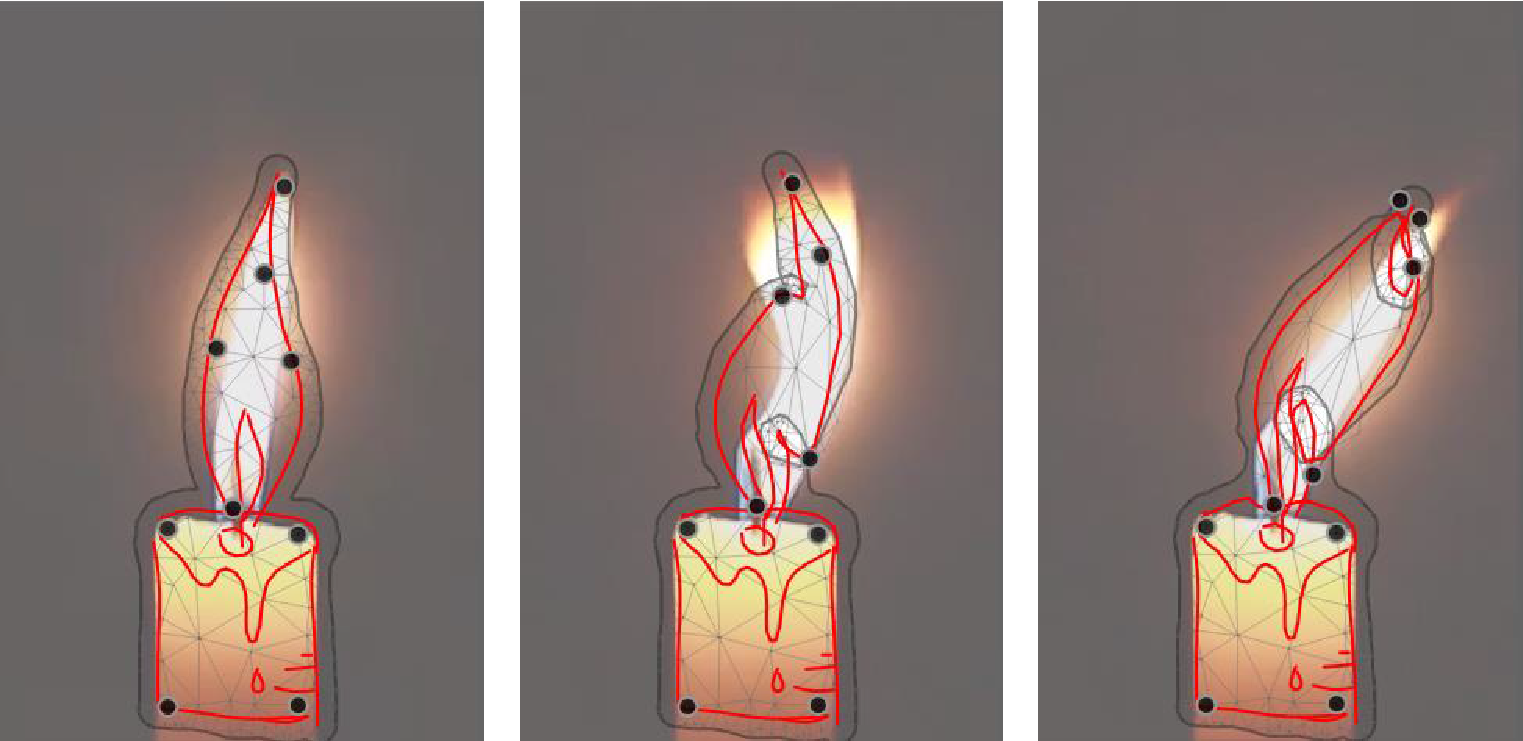
\includegraphics[width=0.85\linewidth]{images/distortion}
	\caption{}
	\label{fig:distortion}
\end{figure}

We thus use a graph tracking method to jointly localize the control points in each frame of the video to extract the object motion, while preserving their geometric structure. Below we first describe how we set up this graph, followed by how to track it through video as solving an energy minimization problem. 

\subsubsection{Graph Setup }

	Denote the sketch structure graph as $ \mathcal{G} = (\mathcal{V}, \mathcal{E}) $, where $ \mathcal{V} $ is the set of control points, and $ \mathcal{E} $ is a set of edges between control points. 
	%It includes a subset of Delaunay triangulation edges of points in $ \mathcal{V} $, and also contain edges that are manually specified by the user, as we will discuss in Sec.~\ref{sec::uat}.
	We initialize $\mathcal{E}$ by applying  Delaunay triangulation on control points, and then exclude those that cross the sketch shape boundary, which is computed from the sketch region extracted in Sec.~\ref{feature_extraction}. We also allow manually specified edges, as  as we will discuss in Sec.~\ref{sec::uat}.	

For each feature point in the current frame, we first determine a candidate set of matches on the next frame. To find a validate candidate set, we use a state-of-the-art object tracking method Struck~\cite{6126251},  which is a tracking-by-detection approach that applies an online-learned SVM (Support Vector Machine) classifier to all image patches in a large window around the current patch $P_i$. The radius of the search window is set to $2r_0$ in our system. 
Intuitively, the classifier treats the supporting region of a control point as an object and tries to detect the same object in a large window around its current position in the next frame. 
The SVM classifier outputs an appearance similarity score for each candidate position, denoted as $\mathbf{a}_i$, and we select the top $K$ of them ($K=10$ in our system) as the candidate match set. 
Formally, we denote the candidate set of the $i$-th point as $ C_{ij}  = \{\mathbf{x}_{ij}, r_{ij}, \mathbf{a}_{ij}\}$, $j = 1, 2, \ldots, K $,  with their appearance similarity scores $\mathbf{a}_{ij}$ in a descending order. 

\subsubsection{Optimization Objective}

Our structure-preserving tracking method solves an energy optimization problem comprising two energy terms:
the {\em appearance energy} $ E_a(C_{ij}) $ that measures the appearance dissimilarity between $C_i$ and its $j$th candidate on the next frame, defined simply as $E_a(C_{ij}) = -\mathbf{a}_{ij}$. 
%  is computed for each tracking feature point using existing tracking methods such as Struck~\cite{6126251}
The {\em structure energy} $ E_s(C_{ip}, C_{jq}) $ measures the lcal structure deformation relative to the initial object shape, if we choose $p$th candidate for $C_i$ and $q$th candidate for $C_j$. It is defined as:
	\begin{align}\label{eq:structure_energy}
		E_s(C_{ip}, C_{jq}) = \|(\mathbf{x}_{ip} -  \mathbf{x}_{jq}) - (\mathbf{x}^1_{i} -  \mathbf{x}^1_{j}) \|^2,
	\end{align}
where $ \mathbf{x}^1_{i} $ and $ \mathbf{x}^1_j $ denote the initial positions of the two control points on the first frame.
This energy measures the edge-length change between the two control points relative to their initial positions. The total energy to be minimized for tracking is then defined as follows:
	\begin{align}\label{eq:total_energy}
		E=\sum_{C_{ij} \in \mathcal{V}}E_a(C_{ij}) + \alpha \sum_{(C_{ip}, C_{jq}) \in \mathcal{E}}E_s(C_{ip}, C_{jq}),
	\end{align}
where $\alpha$ is a balancing weight that is set to \ca{$xxx$} in our system. 

\subsubsection{Energy Minimization}

Given that each control point has ${K}$ tracking candidates, a straightforward solution to minimize the tracking energy is exhaustive search. However it is not scalable when the number of control points is large. We observe that in the tracking process, the best tracking candidates for most control points are correct, and tracking errors such as drifting typically only happen to a small number of points. Based on this observation, we propose an iterative gradient decent method that is much faster to compute and works well in practice. 

We first simply choose the best candidate with the minimal appearance energy for each point, i.e., $C_{i1}$ for the $i$-th point.   
For each point, we compute its sub-graph energy as $E(C_{i1}) = E_a(C_{i1}) + \alpha \sum_{(C_{i1}, C_{j1}) \in \mathcal{E}} E_s(C_{i1}, C_{j1})$. We find the point that has the maximum energy, and minimize it by searching through its other candidates. Intuitively, in every iteration we find the ``worst'' tracking point first, and adjust its position based on its neighbors, under the assumption that the majority of its neighbors are in good positions. We repeat this process until no point can be further adjusted. 

	%Because tracking each feature independently may lead to undesired structure distortion, we preserved several candidates for each point from the tracking samples of small appearance energy.  So this could be formulated as a energy minimization problem over all candidate combinations in $ \mathcal{K} = \{\mathbf{K} | \mathbf{K} = (C_{1j_1}, C_{2j_2},\ldots, C_{nj_n})\} $
	%
	%\begin{align}\label{eq:motion_min}
	%\mathbf{K}^* = \arg\min_{\mathbf{K} \in \mathcal{K}} \sum_{i} E(C_{ij_i}|\mathbf{K})
	%= {\arg}\min_{\mathbf{K} \in \mathcal{K}} \sum_{i} E_t(C_{ij_i}|\mathbf{K}) + \alpha E_s(C_{ij_i}|\mathbf{K})
	%\end{align}
	%
	%, where $ E_s = \sum_{(i, j) \in \mathcal{E}} \Delta d$ is measured by the edge length and angle difference regarding to initial object position.
	%
	%However, 1) it requires searching exponentially many configurations; 2) some candidates may break the structure even if they may have small appearance energy. Therefore, we will propose a method based on graph matching that could avoid the two problems(Algorithm~\ref{alg:motion_extraction}).  
	%Algorithm 1~\ref{alg:motion_extraction} summarizes the algorithm. 
%	Algorithm 1 summarizes the algorithm. 
	
	\begin{comment}
	\begin{algorithm}
		\caption{Motion Extraction}\label{euclid}
		%\label{alg:motion_extraction}
		
		\begin{algorithmic}[1]
			\Require Video $ V $, Feature points $ \mathbf{P}^1 = \{P^1_i | P^1_i = (\mathbf{x}^1_i, r^1_i)\} $ at the first frame.
			
			\Ensure Structure-preserving tracking result $ \mathbf{P}^t = \{P^t_i | P^t_i = (\mathbf{x}^t_i, r^t_i)\} $ for each frame.
			
			\State Construct the structure graph $ \mathcal{G} = (\mathcal{V}, \mathcal{E}) $.
			
			\For {$ t = 2 : m $}
			\LongState{Extract the candidate set for each feature point: $ \mathbf{C}_i  = \{C_{ij}\} $ where $ C_{ij} =
				(\mathbf{x}_{ij}, r_{ij}), j = 1, 2, \ldots, n_i$}.
			
			%\State Initialization: $ \mathbf{P}^t \gets (C_{11}, C_{21}, \ldots, c_{n1}) $
			
			\LongState {Find the best candidate configuration $ \mathbf{K}^* = (C^*_1,\ldots,C^*_n) $ by \ca{selecting} the best candidate for each feature point that minimizes the structure energy (Eq.~\ref{eq:structure_energy}). The drifting feature points $  \mathbf{S} = \{i | E(C^*_i|\mathbf{K}^*) > \eta \} $ are also detected. $ \forall i \notin \mathbf{S}, P^t_i \gets C^*_i. $}
			\LongState {Predict the drifting points' positions $ \{ P^t_i | i \in \mathbf{S}\} $ from spatial neighbors in motion transfer step.} 
			\EndFor
			
			\State {Refine} the positions of drifting points $ \{ P^t_i | i \in \mathbf{S}\} $ according to their global motion trajectory.
			
			\State \Return $ \{\mathbf{P}^t\} $.
			%		\While {true}
			%		\State $ i^* \gets \max_i E_t(C^*_i) + \alpha E_s(C^*-C^*_i) $
			%		\State $ j^* \gets \min_j E_t(c_{i^*j}) + \alpha E_s(C^*-C^*_{i^*} + c_{i^*j}) $
			%		
			%		\EndWhile
			%		
			%		\State $\textit{stringlen} \gets \text{length of }\textit{string}$
			%		\State $i \gets \textit{patlen}$
			%		\If {$i > \textit{stringlen}$} \Return false
			%		\EndIf
			%		\State $j \gets \textit{patlen}$
			%		\If {$\textit{string}(i) = \textit{path}(j)$}
			%		\State $j \gets j-1$.
			%		\State $i \gets i-1$.
			%		\State \textbf{goto} \emph{loop}.
			%		\State \textbf{close};
			%		\EndIf
			%		\State $i \gets i+\max(\textit{delta}_1(\textit{string}(i)),\textit{delta}_2(j))$.
			%		\State \textbf{goto} \emph{top}.
			%		\State \Return $ C $
			
		\end{algorithmic}
	\end{algorithm}
	\end{comment}
	
	%\begin{figure}[t]
	%	\centering
	%	\includegraphics[width = 0.95\linewidth]{algorithm}
	%	\caption{}
	%	\label{fig:mesh}	
	%\end{figure}
	
	
	
	%Existing related work that try to resolve this problem, such as single or object tracking using geometric model~\cite{Martinez20083682,Artner20111969,6243144,6934993,zhang2013structure}, which could tolerant some drifting problems or matching errors. However, these methods usually used a global optimization for all parts/objects, which may lead to either a global drifting problem when using strong structure constraint, or structure distortion at some parts/object because of using strong appearance trackers. 
	%Our method is different with structure-preserving previous single/multiple object tracking methods. 
	
	
	%The structures used in existing multiple object tracking methods\cite{Zhang:2013} is different with ours. 
	%Existing multi-object tracking methods are typically more flexible and do not have as strong structure \ca{among features} as \ca{single object} in our application. Furthermore, most of them are one-step tracking methods that do not correct positions when drifting occurs \ref{XXX}.
	
	%methods~\cite{Martinez:2008,Artner:2011,Cehovin:2013,Cai:2014,Zhang:2013}, including the structure preserved multi-object tracking methods, our method is a detection and correction two-step method. It insures to avoid sketch distortion after the motion is transfered. 
\begin{figure}[t]
	\centering
	\includegraphics[width=1.0\linewidth]{images/trackinginterpolation}
	\caption{Handling difficult tracking cases. Top row: Struck [Hare et al. 2011] fails to track the left front leg of the lion. Middle row: our automatic method better preserves the graph structure, but still looses track on frame 11 due to appearance ambiguity. Bottom row: The user can correct tracking errors by manually editing sparse keyframes. \qingkun{The positions of the control points is specified by the user in the 11st frame(labeled with red).}}
	\label{fig:trackinginterpolation}
\end{figure}
	
\subsubsection{User-Assisted Tracking}\label{sec::uat}

In our experiments, we found that the proposed graph tracking method works better than previous point tracking methods that do not consider the structural relations among the points being tracked. Comprehensive comparisons will be provided in Sec.~\ref{}.
However, given that motion tracking in video is a long-standing computer vision problem, it is unlikely that our proposed tracking method can work perfectly in every situation. 
To handle difficult cases, our system involves the user in the loop to provide necessary guidance.

Firstly, the user can specify geometric constraints between any pair of control points based on their physical properties that cannot be inferred from the video alone. Such an example is shown in Fig.~\ref{}. \qingkun{To-Do: provide an example}

Secondly, the user can correct any drifted tracking point on any frames. For corrected points, the system will replace their automatic tracking positions with the interpolated ones from the user-specified keyframes. We then fix these points as the hard constraints, and re-apply the energy minimization procedure to adjust the positions of the other points. In this way, user edits are propagated both spatially and temporally for quick convergence. An example is shown in Fig.~\ref{fig:trackinginterpolation}, \qingkun{figure is updated} in witch there is a great degree of appearance ambiguity when the two front legs of the lion overlap. While our automatic method (middle row) better preserves the graph structure than the Struck method~\cite{6126251} (top row), it loses track on frame 11. With user's correction on sparse keyframes (frames 5, 11 and 24), our system is able to correctly track the left front leg in the whole sequence. \hongbo{better show a video example as well}



\subsection{Motion Transfer} \label{motion_transfer}
	
After tracking is done, we use the sparse control point trajectories to drive the final sketch animation. 
For this purpose, we first generate a mesh by triangulating the sketch region obtained in Sec.~\ref{feature_extraction}, 
and then use a mesh deformation method to warp the mesh for animation.
Our expectation for the deformation is twofold. 
Firstly, the deformed mesh should closely follow the guidance of the control points to preserve the extracted motion. 
Secondly, the original sketch strokes should not be distorted too much after deformation, otherwise the strokes become unnatural. 

Traditional controlled mesh deformation methods such as the as-rigid-as-possible (ARAP) mesh deformation are only designed to keep the rigidity of the mesh triangles (see Fig.\ref{fig:mesh}), but do not necessarily preserve the shape of the embedded strokes. \hongbo{Need an example to compare the original and modified ARAP methods. }
To solve this problem, we derive a variant of the ARAP method called {\em Sketch-preserving ARAP}. 
Our method includes new mesh triangles derived from user strokes and combines them with the original deformation mesh to preserve stroke shape. %\hongbo{the reviewer might ask what if you use constrained Delaunay triangulation. that is, the stroke points are used to constrain the triangulation?}
The original mesh is denoted as $ \mathcal{M}_0 = (\mathcal{V}_0, \mathcal{T}_0) $, as shown in gray in Fig.~\ref{fig:mesh}.
We uniformly sample points from user strokes, and construct a \textit{sketch triangle} set $\mathcal{M}_s = (\mathcal{V}_s,\mathcal{T}_s) $, by connecting every three consecutive points on each stroke, excluding degenerate triangles on line segments (purple triangles in Fig.~\ref{fig:mesh}). We then construct a \textit{link triangle} set $\mathcal{T}_l$, by connecting each vertex in $\mathcal{V}_s $ with the three vertices of the triangle in $\mathcal{V}_0$ that it falls into.

\begin{figure}
	\centering
	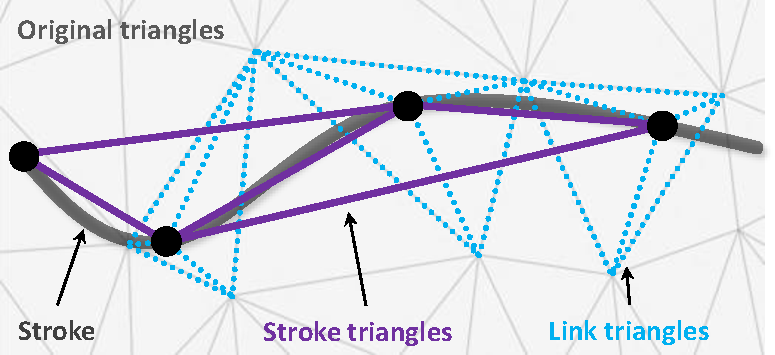
\includegraphics[width=0.85\linewidth]{images/mesh}
	\caption{The modified mesh using for stroke preserving mesh deformation.}
	\label{fig:mesh}
\end{figure}


Given the augmented mesh structure $\mathcal{M}=(\mathcal{V}_0 \cup \mathcal{V}_s, \mathcal{T}_0\cup \mathcal{T}_s\cup \mathcal{T}_l)$, we formulate the stroke-preserving ARAP deformation as the following energy minimization problem: 

\begin{align}\label{eqn:deformationE}
	\min_\mathcal{M} \ E_0 + \beta E_{link} + \gamma E_{sketch},
\end{align}
where $ E_0 $ is the deformation energy of the original mesh $ \mathcal{M}_0 $; $ E_{link} $ and $ E_{sketch} $ are the deformation energy terms of the newly constructed triangle sets $\mathcal{T}_l $ and $\mathcal{T}_s $, respectively. 
Specifically, following \cite{Igarashi:2005}), for each triangle set, we have:
\begin{align}
 E(\mathcal{T}) = \sum_{t\in \mathcal{T}} \sum_{v_i, v_j \in t} \|\overrightarrow{v'_iv'_j} - H\overrightarrow{v_iv_j}\|^2 ,
 \end{align}
  where $ H $ is a rigid transformation matrix that is achieved by a two-step optimization algorithm; please refer to \cite{Igarashi:2005} for more details.
The same definition of $E(\mathcal{T})$ is applied to $\mathcal{T}_0, \mathcal{T}_{link}, \mathcal{T}_{sketch}$.
 Minimizing $ E_{sketch} $ keeps the shape of the strokes while minimizing $ E_{link} $ transfers the deformation of the original mesh to the strokes. 
In our system, we set the weight $ \beta $ to be a small value of 0.01, as we allow the triangles in the link triangle set to be distorted to balance between deformation and sketch shape preserving. We set $ \gamma = 1$ by default in order to better preserve the sketch shape. 

{\bf User-specified local rigidity.} 
The energy defined in Equation~\ref{eqn:deformationE} applies the same shape preserving weight $\gamma$ to all sketch strokes. In our experiments we have found that sometimes it is desirable to have parts of the sketch to be more rigid, while making other parts more flexible to capture larger motion. For example, imagine animating a standing dog wagging his tail \hongbo{I'm expecting this dog example in the video}. \qingkun{Figure~\ref{fig:deformationcomparison}} The user may want to apply a stronger rigidity constraint on the dog's body to eliminate tracking noise, but a weaker rigidity to his tail part to better capture the intensive motion.
We thus allow the user to use a local rigidity brush to quickly specify strokes that need to be more rigid. 
All the strokes that are under the brush will have the corresponding $ \gamma $ value increased by a factor greater than one. The brush is also accumulative so the more the user brushes, the more rigid that the underlying sketch strokes will be. 
%\Jue{An example is shown in the accompanying video.}

\begin{figure}
	\centering
	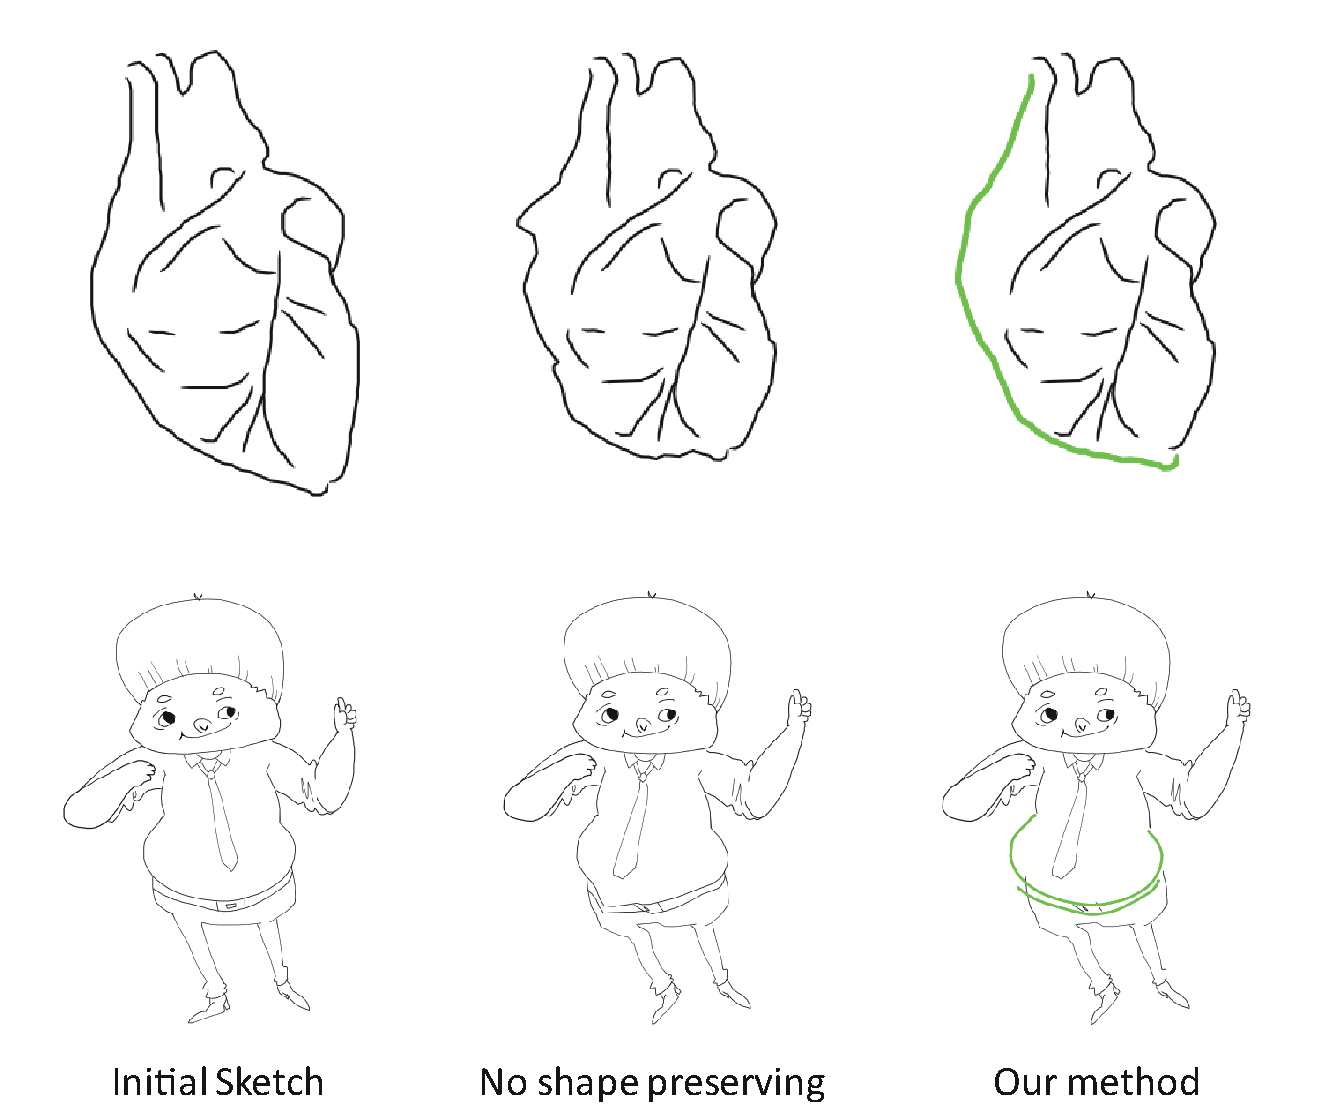
\includegraphics[width=0.85\linewidth]{images/deformationcomparison}
	\caption{Sketch deformation results with/out shape preserving method.}
	\label{fig:deformationcomparison}
\end{figure}

\subsection{Extensions}

\qingkun{To reuse the extracted motion, we also extend it for sketches that are not similar to video objects. The main goal is to map the original key points of the video to the new sketch. This could be solved by finding the matching between the original sketch and the new one. 
	
We first obtain the sketch contours, $ s_o, s_n $, of the original and new sketches using the method in \ref{motion_extraction}. Then we sample $ k_0 $ and $ k_n $  points, $ \textbf{P} = \{p_i\} $ and $ \textbf{Q} = \{q_i\} $, inner the two contours. Then the correspondence could be obtained by finding the affine transformation $ T $ between the two point sets by ICP point matching methods. Then for any point $ x_o $ inner $ s_o $, we could find the corresponding position $ x_n $ inner $ s_n $ by   Given a key point's position of the first frame, $ x_i $, we first compute $ k $ nearest points in $ P $ and its corresponding points in $ \textbf{Q} $. Then the corresponding position $ x_n $ could be computed by the berry centric weight of the $ k $ points of $ \textbf{Q} $. If $ x_n $ is located outside of $ s_n $, then we remove one point from the $ k $ points and re-compute the position until $ x_n $ is located inside of $ s_n $.
}



\section{Evaluation}
\qingkun{To-Do}
%Our system aims at providing the user with an easy way to add 3D strokes to an existing shape for communicating conceptual design ideas. Strokes drawn by a user over an existing 3D shape are generally of two types. The first type lie on an existing surface. The 3D information for such a stroke can be determined easily by projection onto the surface. The second type of strokes are drawn to specify a non-existent part of the shape, indicating how the original shape is to be modified. Determining the 3D information for this type of stroke is nontrivial. Our system focuses on providing an interface to draw sketch strokes of the second type.

%We will conduct a user study to evaluate our system. The user study will consist of two parts. In User Study I, a number of participants will be invited to use both our system and an existing state-of-the-art keyframe method such as Adobe Animator to create two animations for every given pair of sketch and video. 
%To evaluate the efficiency of our system, 
%%In this experiment, the participants will be asked to create a sketch animation to a given video. 
%we will compare the completion time and the number of operations which include the sketching operations and the editing operations. 
%The participants will also be asked to answer a questionaire on the usability of our system. 
%
%The sketch animations created using the two methods will then be evaluated by a different group of participants in User Study II.
%We will ask the participants to score each sketch animation created in User Study I on aesthetics, completeness, etc. 


\begin{figure}
	\centering
	\includegraphics[width=0.9\linewidth]{images/trackingcomparison}
	\caption{}
	\label{fig:trackingcomparison}
\end{figure}

\section{Results}


% Please add the following required packages to your document preamble:
% \usepackage{multirow}
\begin{table*}[]
	\centering
	\caption{My caption}
	\label{my-label}
	\begin{tabular}{l|cc|cc|cc|cc|cc}
		\hline
		\multirow{2}{*}{} & \multicolumn{2}{c|}{\textbf{OURS}} & \multicolumn{2}{c|}{\textbf{STRUCK}} & \multicolumn{2}{c|}{\textbf{SPOT}} & \multicolumn{2}{c|}{\textbf{SAMF}} & \multicolumn{2}{c}{\textbf{DT}} \\
		& \textit{Err.}    & \textit{Pre.}   & \textit{Err.}     & \textit{Pre.}    & \textit{Err.}    & \textit{Pre.}   & \textit{Err.}    & \textit{Pre.}   & \textit{Err.}  & \textit{Pre.}  \\ 
		\textbf{Candle}   & 0.999            & 0.982           & 36.451            & 0.675            & 13.439           & 0.786           & 28.552           & 0.737           & 35.962         & 0.615          \\
		\textbf{Cartoon}  & 1.806            & 0.940           & 3.731             & 0.884            & 7.206            & 0.759           & 5.217            & 0.801           & 7.397          & 0.744          \\
		\textbf{Fish}     & 3.537            & 0.820           & 13.600            & 0.587            & 25.516           & 0.179           & 43.196           & 0.434           & 43.525         & 0.345          \\
		\textbf{Kangaroo} & 4.574            & 0.805           & 12.598            & 0.666            & 19.727           & 0.427           & 44.419           & 0.282           & 21.830         & 0.415          \\
		\textbf{Kite}     & 6.534            & 0.727           & 21.293            & 0.465            & 9.435            & 0.618           & 13.159           & 0.663           & 28.399         & 0.404          \\ \hline
	\end{tabular}
\end{table*}
\qingkun{To-Do}
%We will extend the basic \textit{Live Sketch} to two applications.
%%	\textbf{Many-to-one motion transfer}
%Segmenting a character into meaningful parts or layers and animating them separately is common in animation creation. Similarly, our system will also allow transferring motions from multiple videos to different parts of a single sketch. Independent motion transfer for each part will lead to spatial inconsistency, which can be solved by existing motion retargeting method such as AniMesh~\cite{Jin:2015}.
%Another way to increase the usability of motions is to transfer motions to a sketch in different temporal intervals.  We will need to address the issue of smooth transitions between motions.
%Note that in such scenarios the number of control points used in the two motions may be different but the original mesh is the same as
%the two motions are transferred to the same sketch. 
%%the two sets of control points positions between the two control point sets at the transition position may not be well aligned and may locate at different parts of the sketch. 
%A possible solution to attain smooth transition from motion A to motion B is as follows (see Figure 6). We first compute the position of each control point of A on B's deformed mesh by mesh interpolation. Next we can find a new motion trajectory for each point of motion A during B's time interval. A smooth transition trajectory can easily be found between the two trajectories by Hermite 
%interpolation.
%by Laplacian smoothing after connecting them. 
%Similarly, we can obtain a smooth transition trajectory for each control point of motion B. Therefore, the animation can be transited smoothly based on the transition trajectories.

%Interactive illustrations can provide a more playful or informative experience~\cite{Kazi:2014b}. We will also extend our \textit{Live Sketch} tool to achieve dynamic interactive animations. Users can interact with the animation to control its playback direction, speed of playing and locally deform near a dragged point. 
%We will provide a user interface that when the user drags one part of the sketch, the animation will be played forward or backward according to the drag direction with respect to the nearest motion trajectory. The speed of playing will depends on the cursor speed.  The point on the sketch where it is being dragged will be deformed such that it stays attached to the cursor. This can be achieved by applying a sketch deformation method described in Task D, where the drag point is treated as an additional control point.
%% (user is also required to give another static point). 
%Different dynamic motion constraints can also be specified to different parts, for example, producing the effect of magnifying the motion of certain parts while suppressing the motion of the other parts. 
%Furthermore, dynamic dragging constraints can also be applied to simulate effects such as flowers being blown by wind.  

%It also allow user to add an external force like wind with dynamic direction and speed.
%We provide a user interface that when user drag some part of the sketch, the animation would be played adaptively and dynamically and also respect to user's dragging position. The animation speed and direction can be computed by the dragging speed and direction. To make sure that the dragging part is always attached to the cursor, a sketch deformation is applied to the deformed sketch using the method in Task D, where the dragging point is treated as the control point (user is also required to give another static point). Furthermore, our system can also produce dynamic animation when user specifies dynamic dragging constraints such as the wind, or highlights the motion of some parts by magnifying its motion and reducing others'.

%
%\subsection{Extensions}
%
%Our tool aims to animate a sketch using the same motion of the object in the video, it thus will look as real as in the video. Since the users might want to produce a stylized animation, we will provide post-animation stylization tools, such as using animation filters~\cite{Wang:2006}, applying the 12 animation principles~\cite{Kazi:2016}, and adding animation looping.
%
%%{The methodology described above focuses on motion transfer for a single object.} An extracted motion can also be re-used and transferred to multiple objects.  In that case, motion re-targetting is necessary. 
%
%%We will also investigate creation of sketch animations containing numerous objects. For this purpose, we will need to design and implement a new user interface that can combine the results of several animation results of our method into one scene.
%
%Sketching on touch-based devices is direct and natural. Hence,
%implementing Live Sketch on devices like iPad and iPhone will be highly desirable.  This will require redesigning the user interface to improve user experience on sketching and interactions, such as integrating multitouch features and stylus pen.

%In our system, we require only coplanar strokes be drawn in each step. This setting ensures that our system is able to generate the expected 3D sketch with only simple interaction. However, this restriction may hinder the user during drawing. The ultimate goal of allowing the user to draw strokes on arbitrary planes or surfaces in any order is too difficult. Instead, we will further investigate how to make our system more general by introducing other type of constraints besides the coplanar constraint for drawing strokes, constraining the current set of drawn curves to be on a curved surface, or to be symmetric. 
%%\ca{Similar to the current algorithm, we will borrow the geometry information to constrain the drawn curves. Specifically, 
%If the matched sharp edges are on a common curved surface that is extracted from the shape, the surface is a potential canvas. If the drawn strokes are self-symmetrical after an affine transformation, the canvases that realize this transformation might be desirable ones. When the user draws a set of strokes, it is unknown which constraint should be used. A possible solution will be to traverse all the constraints and generate all possible candidate 3D strokes which will be ranked using the same criteria described before.

%An issue to solve then would be how does the system automatically recognize what type of constraint to enforce on the drawn strokes. \ca{Possible solutions? curved surface derived from the given shape}

%Man-made shape is the main focus of our system. It is because designing man-made shapes is more common than organic shapes. 
%For example, the user may want to modify the design of an existing furniture model, or change the appearance of a building model. When designing a 3D scene, the models in this scene are mostly man-made. In our system, we will mainly focus on the following information.




%\section{Methodology}
%The pipeline of our system is shown in Fig~\ref{overview}. Given two inputs sketch and the video, our method contains three main steps to animate the static sketch $ \mathcal{S} $:
%
%\begin{description}
%	\item[Video\&Sketch Alignment.] Alignment between the sketch (vector graphics) and video frame (bitmap image) is very hard. We proposed a method that extracts the feature points both good to track in video and in the region of user's interest in sketch.
%	\item[Motion Extraction.] Drifting problem is always hard to avoid in video tracking, which could produce unexpected animation results. We present a   tracking method that keeps the object structure even when some parts drifts at some frames.
%	\item[Motion Transfer.] With the correspondence and the extracted video motion, we animate the sketch using a stroke-preserving as-rigid-as possible mesh deformation method. This method could keep the stroke shape well even with large deformation. 
%\end{description}
%
%\begin{figure*}[t]
%	\centering
%	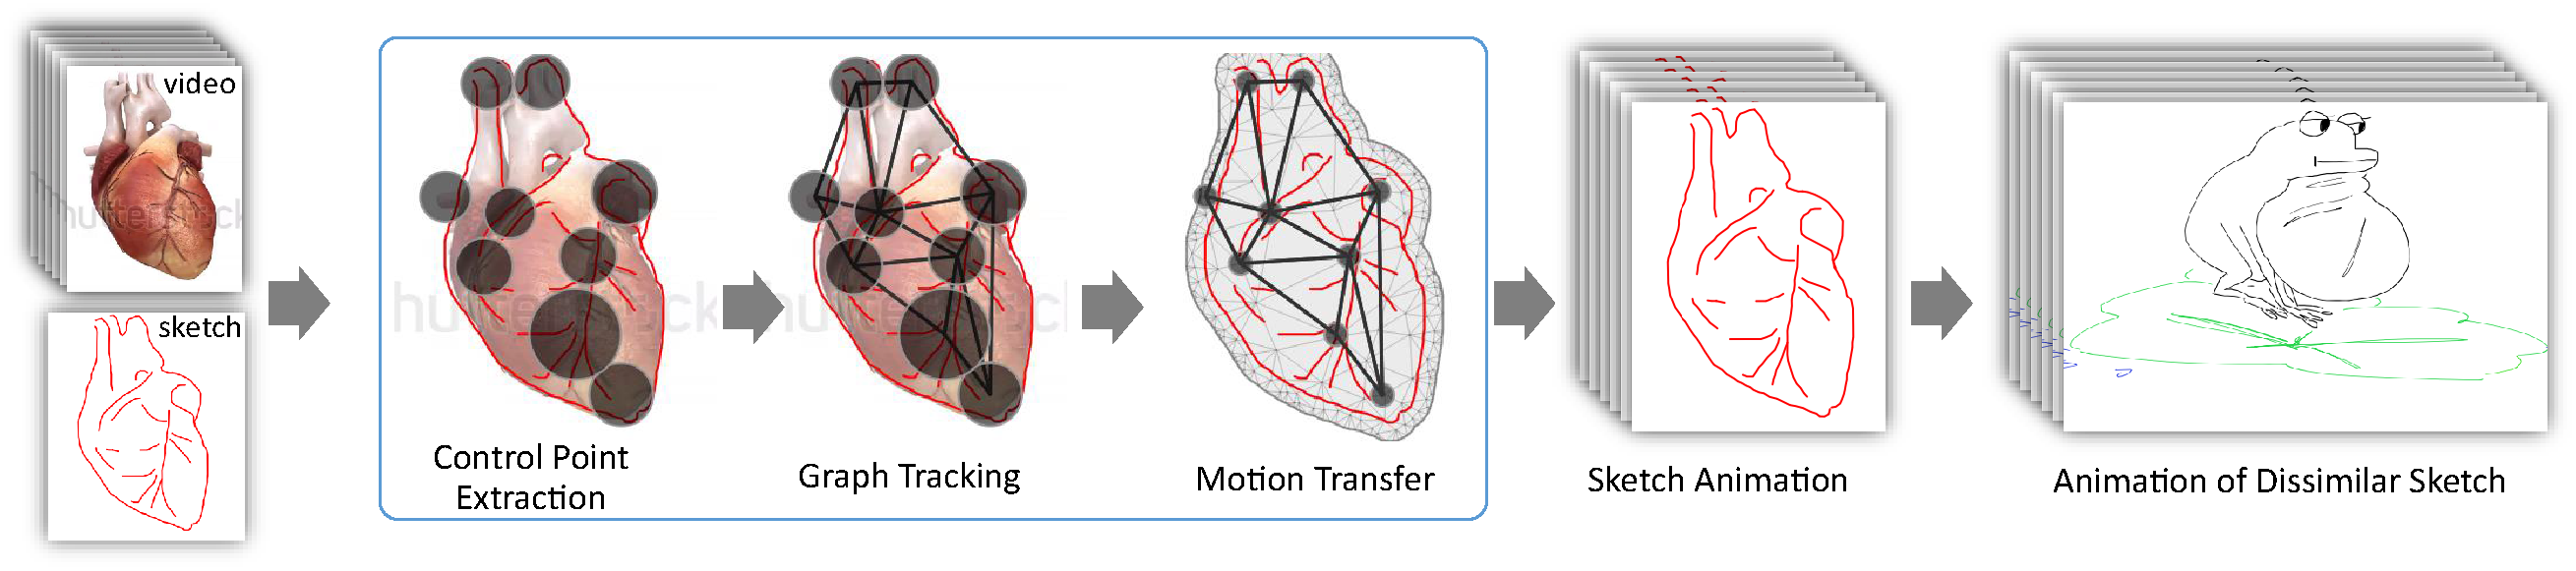
\includegraphics[width = 0.95\linewidth]{images/overview}
%	\caption{Given the sketch and the video, the first step alignment would try to extract some good feature points from video and sketch and compute their correspondence.
%		Then we extract the motion by tracking the good feature points of the video by using object structure.		
%		Combined with the correspondence and the motion, we used a stroke-preserving ARAP method to transfer the motion to the sketch.
%		After the three steps, the final sketch animation is generated. 
%	}
%	
%	\label{fig:overview}	
%\end{figure*}
%
%\subsection{Video\&Sketch Alignment}\label{alignment}
%Finding the correspondence between video and sketch is tough problem, because the latter is more abstract and semantic. Therefore, we need to extract the feature points that are both good to track for video and good to control for sketch.
%
%We first extract the good feature to control for sketch and to track of the first video frame by scale irrelevant corner detection method[XXX]. Then a graph matching is used to find the best one-to-one mapping between the two feature point set [XXX].
%
%However, sometimes it would be hard or even impossible to detect the correspondence, because the sketch and the video object do not have similar structure (see the example in Fig. [XXX]). we also provide a user interface to edit the flexible correspondence. 
%
%\begin{figure}
%	\centering
%	\includegraphics[width=0.85\linewidth]{C:/Users/suqin/Documents/flexible}
%	\caption{}
%	\label{fig:flexible}
%\end{figure}
%
%
%\subsection{Motion Extraction}\label{motion_extraction}
%The goal of this step is extract robust motion for each feature point that is extracted in previous step. We proposed a method that could 
%1)track the object that could preserve its structure 2) keep the structure by using the structure even if drifting problem happens at some parts.
%Unlike previous graph-based or structure-preserving object tracking methods, our method could detect the drifting parts and predict its positions by spatial and temporal neighborhood.
%Our structure preserved object tracking method mainly considers two part: 1) $ E_t $ appearance energy that existing tracking methods 2) $ E_s $structure energy that measures the structure deformation. Assuming that we could obtain several candidates for the $ i $th part, $ \{ c_{ij} \} $ ($ c_{ij} $ is contains the candidate position $ p_{ij} $ and same size with initial frame), with appearance energy ascending order. So this could be formulated as a energy minimization problem
%\[ E* = \min_{C \in \mathcal{C}} E_t(C) + \alpha E_s(C) \]
%over all candidate configurations in $ \mathcal{C} $, where $ E_s = \sum_{e} \Delta d + w\sum_{\theta} \Delta \theta$ is measured by the edge length and angle difference regarding to initial object position.
%
%However, 1) it requires searching exponentially many configurations; 2) some candidates may break the structure even if they may have small appearance energy. To solve this problem, we will propose a method that could detect the bad candidates, preserve the global structure by the good ones and then predict the positions by its spatial and temporal neighborhood.
%
%%\begin{algorithm}
%%	\caption{Motion Extraction}\label{euclid}
%%	\begin{algorithmic}[1]
%%		\Procedure{MyProcedure}{}
%%		\State Initialize: $ C^* \gets (c_{11}, c_{21}, ..., c_{i1}, c_{n1}) $
%%		
%%		
%%		\While {true}
%%		\State $ i^* \gets \max_i E_t(C^*_i) + \alpha E_s(C^*-C^*_i) $
%%		\State $ j^* \gets \min_j E_t(c_{i^*j}) + \alpha E_s(C^*-C^*_{i^*} + c_{i^*j}) $
%%		
%%		\EndWhile
%%		
%%		\State $\textit{stringlen} \gets \text{length of }\textit{string}$
%%		\State $i \gets \textit{patlen}$
%%		\If {$i > \textit{stringlen}$} \Return false
%%		\EndIf
%%		\State $j \gets \textit{patlen}$
%%		\If {$\textit{string}(i) = \textit{path}(j)$}
%%		\State $j \gets j-1$.
%%		\State $i \gets i-1$.
%%		\State \textbf{goto} \emph{loop}.
%%		\State \textbf{close};
%%		\EndIf
%%		\State $i \gets i+\max(\textit{delta}_1(\textit{string}(i)),\textit{delta}_2(j))$.
%%		\State \textbf{goto} \emph{top}.
%%		\State \Return $ C $
%%		\EndProcedure
%%		
%%	\end{algorithmic}
%%\end{algorithm}
%
%\subsection{Motion Transfer}\label{motion_transfer}
%
%Motion transfer aims to transfer the extracted motion of video to the sketch by using the extracted correspondence in section \ref{motion_extraction}. The simplest way is using as-rigid-as possible(ARAP) mesh deformation method.
%To generate the mesh that is used to deform the sketch, we triangulate the contour that is obtained by active contour method for the sketch image. Then we can animate the sketch by deforming the mesh with the feature points' position as handles. However, ARAP mesh deformation could not preserve the stroke shape because it only keeps the rigidibility of the mesh triangles (see the example in Fig.XXX). 
%
%Therefore, we proposed stroke-preserving ARAP method to preserve the stroke shape during the mesh deformation.
%Denote the feature positions of the $ t $th and $ (t + 1) $th frame as $ \mathbf{p}^t = \{p^t_{i}\} $ and $ \mathbf{p}^{t+1} = \{p^{t + 1}_{i}\} $.
%To preserve the stroke shape, we reconstruct the original mesh $ \mathcal{M}_0 = (\mathcal{V}_0, \mathcal{T}_0) $ by adding one vertex set $ \mathcal{V}_s $ that includes all the sketch points and two triangle sets $ \mathcal{T}_s, \mathcal{T}_l $, where
%
%\begin{description}
%	\item[Sketch triangle set $\mathcal{T}_s $] is constructed by connecting every three consequent points on each stroke;
%	\item[Link triangle set $\mathcal{T}_l $] is constructed by connecting each sketch point with its outer triangle�s vertices.
%\end{description}
%
%\begin{figure}[t]
%	\centering
%	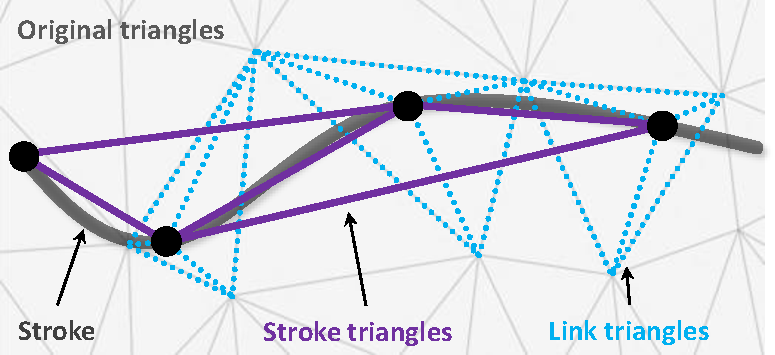
\includegraphics[width = 0.95\linewidth]{images/mesh}
%	\caption{Reconstructed mesh for stroke-preserving ARAP deformation.}
%	
%	\label{fig:mesh}	
%\end{figure}
%
%Then, the ARAP mesh deformation is applied to the new constructed mesh $ \mathcal{M} = (\mathcal{V}, \mathcal{E}) $ where $ \mathcal{V} = \mathcal{V}_0 \cup \mathcal{V}_s $ and $ \mathcal{E} = \mathcal{E}_0 \cup \{e|e\in \mathcal{T}_s \cup \mathcal{T}_l\} $ by the following energy minimization formulation:
%\[ \min E_0 + E_{1ink} + \beta E_{sketch} \]
%, where $ E_0 $ is deformation error of the original mesh $ M_0 $, $ E_{1ink} $ and $ \beta E_{sketch} $ represents the error of the new added triangle sets $\mathcal{T}_s $ and $\mathcal{T}_l $. The main idea of this method is that the original mesh will try to deform the sketch triangles through the intermediate link triangles. If the weight of the stroke triangles are large enough, the shape of the stroke would be preserved. $ \beta $ is set to be 10 in our implementation.
